\chapter{SINS database table}
\label{app:SINS-Databse-Table}
This chapter shows a table with the different activities recorded within the SINS database. The activities are divided into the room where they were recorded.

\begin{table}[htbp]
    \centering
    \caption[SINS database recorded activities for each room]{SINS database recorded activities for each room \footnotemark}
	\label{tab:sins-database-recorded-activities}
    \begin{tabular}{l|l|c|c}
        \toprule
        \textbf{Room} & \textbf{Activity} & \textbf{Nr. ex.} & \textbf{duration (min.)} \\ 
        \midrule[1pt]
        \multirow{10}{*}{Living room} & Phone call & 22 & 8.17 $\pm$ 13.73 \\
        \cline{2-4}
        & Cooking & 19 & 16.62 $\pm$ 9.49 \\
        \cline{2-4}
        & Dish washing & 15 & 6.37 $\pm$ 1.49 \\
        \cline{2-4}
        & Eating & 19 & 7.78 $\pm$ 4.27 \\
        \cline{2-4}
        & Visit & 9 & 13.3 $\pm$ 12.11 \\
        \cline{2-4}
        & Watching TV & 13 & 155.38 $\pm$ 93.28 \\
        \cline{2-4}
        & Working & 15 & 31.24 $\pm$ 39.33 \\
        \cline{2-4}
        & Vacuum cleaning & 15 & 4.79 $\pm$ 2.14 \\
        \cline{2-4}
        & Other & 15 & 0.75 $\pm$ 0.95 \\
        \cline{2-4}
        & Absence & 15 & 66.37 $\pm$ 130.30 \\
        \midrule[1pt]
        \multirow{7}{*}{Bathroom} & Drying with towel & 10 & 1.67 $\pm$ 0.28 \\
        \cline{2-4}
        & Shaving & 13 & 1.91 $\pm$ 1.46 \\
        \cline{2-4}
        & Showering & 10 & 6.11 $\pm$ 2.38 \\
        \cline{2-4}
        & Tooth brushing & 19 & 1.41 $\pm$ 0.25 \\
        \cline{2-4}
        & Vacuum cleaning & 9 & 0.87 $\pm$ 0.59 \\
        \cline{2-4}
        & Other & 75 & 0.42 $\pm$ 0.4 \\
        \cline{2-4}
        & Absence & 35 & 248.56 $\pm$ 263.62 \\
        \midrule[1pt]
        \multirow{3}{*}{Hall} & Vacuum cleaning & 9 & 3.31 $\pm$ 1.11 \\
        \cline{2-4}
        & Other & 164 & 0.36 $\pm$ 0.22 \\
        \cline{2-4}
        & Absence & 175 & 50.17 $\pm$ 102.52 \\
        \midrule[1pt]
        \multirow{3}{*}{Toilet} & Toilet visit & 21 & 4.74 $\pm$ 3.24 \\
        \cline{2-4}
        & Vacuum cleaning & 7 & 0.53 $\pm$ 0.07 \\
        \cline{2-4}
        & Absence & 31 & 282.75 $\pm$ 263.19 \\
        \midrule[1pt]
        \multirow{5}{*}{Bedroom} & Dressing & 28 & 1.53 $\pm$ 1.10 \\
        \cline{2-4}
        & Sleeping & 7 & 348.43 $\pm$ 130.73 \\
        \cline{2-4}
        & Vacuum cleaning & 7 & 1.04 $\pm$ 0.27 \\
        \cline{2-4}
        & Other & 22 & 0.27 $\pm$ 0.23 \\
        \cline{2-4}
        & Absence & 22 & 122.28 $\pm$ 157.43 \\
        \bottomrule
    \end{tabular}
\end{table}
\footnotetext{\fullcite{dekkers_sins_2017}}

\chapter{Milestone reports}
\label{app:Milestone-Reports}
This chapter lists the individual milestone reports. These should provide information on the status of the project during the realisation. For every completed milestone, a report was written before the next phase could be started. The table \fullref{tab:Milestones} shows the milestones within the thesis as well as the corresponding dates when the milestone and the phase will be completed and reviewed. The milestones are also shown in the whole project plan in \fullref{fig:Project-Plan}.

\section{Milestone report M1 from the 15.03.2020}
In the first phase of the project, the main goal was to research the subjects used for the thesis. Within phase, the project also had to be initialised and started. More precisely, the project structure and documentation also had to be defined. The goal was also to finish the first chapter of the thesis \fullref{ch:Related-Work} along with the research.

\begin{table}[htbp]
    \centering
    \caption{Work carried out milestone M1 (15.03.2020)}
	\label{tab:Work-Carried-Out-M1}
    \begin{tabular}{p{.70\textwidth} | p{.20\textwidth}}
        \toprule
        \textbf{Task} & \textbf{Status} \\ 
        \midrule[1pt]
        Research: Dataset & finished \\
        \hline
        Research: Audio processing & finished \\
        \hline
        Research: Triplet Loss & finished \\
        \hline
        Research: Tile2Vec & finished \\
        \hline
        Research: Evaluate research & finished \\
        \hline
        Realisation: Project setup & started \\
        \hline
        Realisation: Input pipeline & started \\
        \bottomrule
    \end{tabular}
\end{table}

\subsection{What work was carried out in the last reporting period}
The tasks carried out within this period are shown in the table \fullref{tab:Work-Carried-Out-M1}, along with the status of the task at the time of the milestone review. A detailed report on the entire tasks carried out within the period is shown in the work journal \ref{tab:Work-Journal}. To reach the goal of simultaneously finishing the chapter \ref{ch:Related-Work} with the research, each researched topic was documented right away. 
\subsection{State of progress}
The current milestone was successfully reached since all the planned tasks could be finished. The phase was finished too early so that the next period could already be started, the realisation phase. 

\subsection{Top three risks including planned measures}
\begin{enumerate}
    \setlength\itemsep{0em}
    \item Formulas related work wrong, will be checked by Daniel Pfäffli
    \item Topics missing in related work, will be checked by Daniel Pfäffli
    \item Input pipeline structure, will be discussed at the next meeting
\end{enumerate}

\section{Milestone report M2 from the 29.03.2020}
In the second milestone of the project, the main goal was to finish the whole project setup. The project repository had to be set up, the input pipeline was created for the dataset, and the default model architecture was created. The purpose was that after this milestone, the project is at a certain point, that the implementation of specific architectures is fast enough to experiment with different ones.

\begin{table}[htbp]
    \centering
    \caption{Work carried out milestone M2 (29.03.2020)}
	\label{tab:Work-Carried-Out-M2}
    \begin{tabular}{p{.70\textwidth} | p{.20\textwidth}}
        \toprule
        \textbf{Task} & \textbf{Status} \\ 
        \midrule[1pt]
        Realisation: Project setup & finished \\
        \hline
        Realisation: Input pipeline & finished \\
        \hline
        Realisation: Default architecture & finished \\
        \hline
        Realisation: Evaluation Workflow & midway \\
        \hline
        Realisation: Unit tests & midway \\
        \bottomrule
    \end{tabular}
\end{table}

\subsection{What work was carried out in the last reporting period}
The tasks carried out within this period are shown in the table \fullref{tab:Work-Carried-Out-M2}, along with the status of the task at the time of the milestone review. A detailed report on the entire tasks carried out within the period is shown in the work journal \ref{tab:Work-Journal}. Two tasks were not completed within the period, which was now prioritised in the next phase and will get completed first. The milestone could not be completed because to little time was planned for tasks like \flqq input pipeline\frqq or \flqq evaluation workflow\frqq. The evaluation workflow was completed except for the classifier, to evaluate the architecture in relation to the other models in the DCASE Challenge. Unit tests were not written for all the created models but will be right away at the start of the next milestone.

\subsection{State of progress}
The current milestone was not reached since two tasks could not be finished entirely. The uncompleted tasks were prioritised and were moved to the next phase of the project.

\subsection{Top three risks including planned measures}
\begin{enumerate}
    \setlength\itemsep{0em}
    \item GPU caching / file deletion problem, will be discussed at the next meeting
    \item Classifier architecture, will be discussed at the next meeting
    \item Unit tests for models, will be discussed at the next meeting 
\end{enumerate}

\section{Milestone report M3 from the 12.04.2020}
The third milestone aimed to finalise the realisation. The idea of unsupervised triplet loss had to be implemented, like the one from Tile2Vec for both datasets. Furthermore, an easy to use architecture for the experiments had to be developed. Thus the experiments should be conducted relatively simple. The main goal is to provide an architecture which is reliable, arbitrarily expandable and repeatable. All of these points are essential for conducting successful experiments.

\begin{table}[htbp]
    \centering
    \caption{Work carried out milestone M3 (12.04.2020)}
	\label{tab:Work-Carried-Out-M3}
    \begin{tabular}{p{.70\textwidth} | p{.20\textwidth}}
        \toprule
        \textbf{Task} & \textbf{Status} \\ 
        \midrule[1pt]
        Realisation: Evaluation Workflow & finished \\
        \hline
        Realisation: Unit tests & finished \\
        \hline
        Realisation: Tile2Vec implementation & finished \\
        \hline
        Realisation: Architecture for experiments & finished \\
        \hline
        Experiments: Conduct experiments & started \\
        \bottomrule
    \end{tabular}
\end{table}

\subsection{What work was carried out in the last reporting period}
The tasks carried out within this period are shown in the table \fullref{tab:Work-Carried-Out-M3}, along with the status of the task at the time of the milestone review. A detailed report on the entire tasks carried out within the period is shown in the work journal \ref{tab:Work-Journal}. Two tasks were not completed during the last phase and were completed at the start of this phase by prioritising them. Both of the other tasks which were planned to complete during this phase were completed.

\subsection{State of progress}
The current milestone was successfully reached since all the planned tasks could be finished. The phase was finished too early so that the next period could already be started, the experiment phase. 

\subsection{Top three risks including planned measures}
\begin{enumerate}
    \setlength\itemsep{0em}
    \item Review evaluation workflow, will be discussed at the next meeting
    \item Review of study doc, will be discussed at the next meeting
    \item Review of test concept, will be discussed at the next meeting 
\end{enumerate}

\chapter{Test concept}
\label{app:Test-Concept}

\clearpage
\landscapevalues

\begin{table}[htbp]
    \centering
    \caption{Test concept}
	\label{tab:Test-Concept}
    \begin{tabular}{p{.15\textwidth} | p{.40\textwidth} | p{.05\textwidth} | p{.15\textwidth} | p{.15\textwidth}}
        \toprule
        \textbf{Test case} & \textbf{Steps} & \textbf{Status} & \textbf{Expected result} & \textbf{Actual result} \\ 
        \midrule[1pt]
        DCASE iterator & 
        \begin{minipage}{5in}
        \vskip 4pt
        \begin{enumerate}
        \setlength\itemsep{0em}
        \item get dataset from model factory
        \item loop over dataset using for loop
        \item check if the entries are not \texttt{None}
        \end{enumerate}
        \vskip 4pt
        \end{minipage} & \cellcolor{green!30!white}passed & entries available & entries available \\
    \hline
        DCASE triplets & 
        \begin{minipage}{5in}
        \vskip 4pt
        \begin{enumerate}
        \setlength\itemsep{0em}
        \item get dataset from model factory
        \item loop over dataset using for loop
        \item for each entry in the dataset load triplets
        \item loop over resulting triplets
        \item check if there are three triplets
        \item check if all constituents have dimension two 
        \end{enumerate}
        \vskip 4pt
        \end{minipage} & \cellcolor{green!30!white}passed & dataset generates valid triplets & valid triplets generated \\
        \bottomrule
    \end{tabular}
\end{table}

\clearpage
\defaultpagestyle

\chapter{Study Doc}
\label{app:Study-Doc}

This chapter contains all of the study docs from the conducted experiments, they include detailed information about each one of the experiments as well as the conclusion out of each.

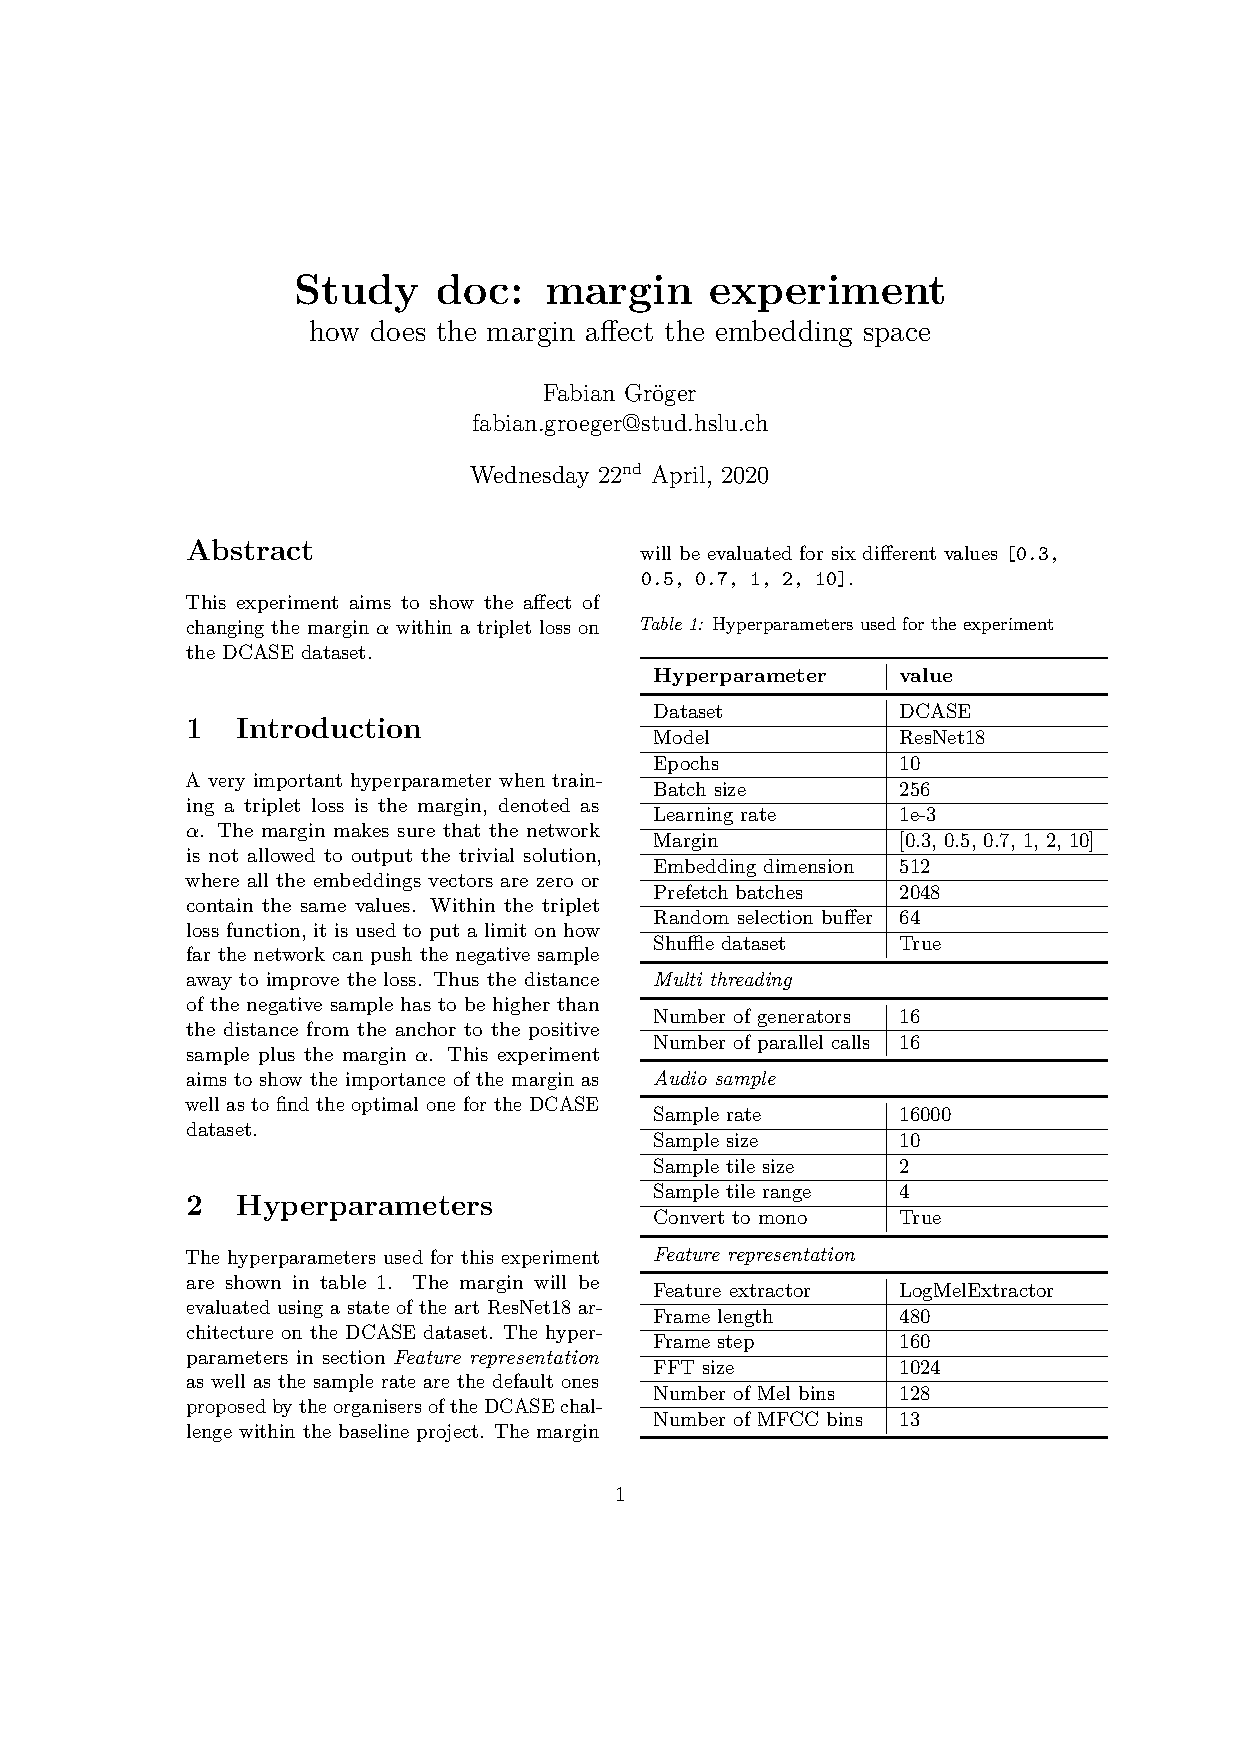
\includepdf[scale=1.0, pages=1-]{study-doc/experiment_margin/Study_Doc_Margin.pdf}

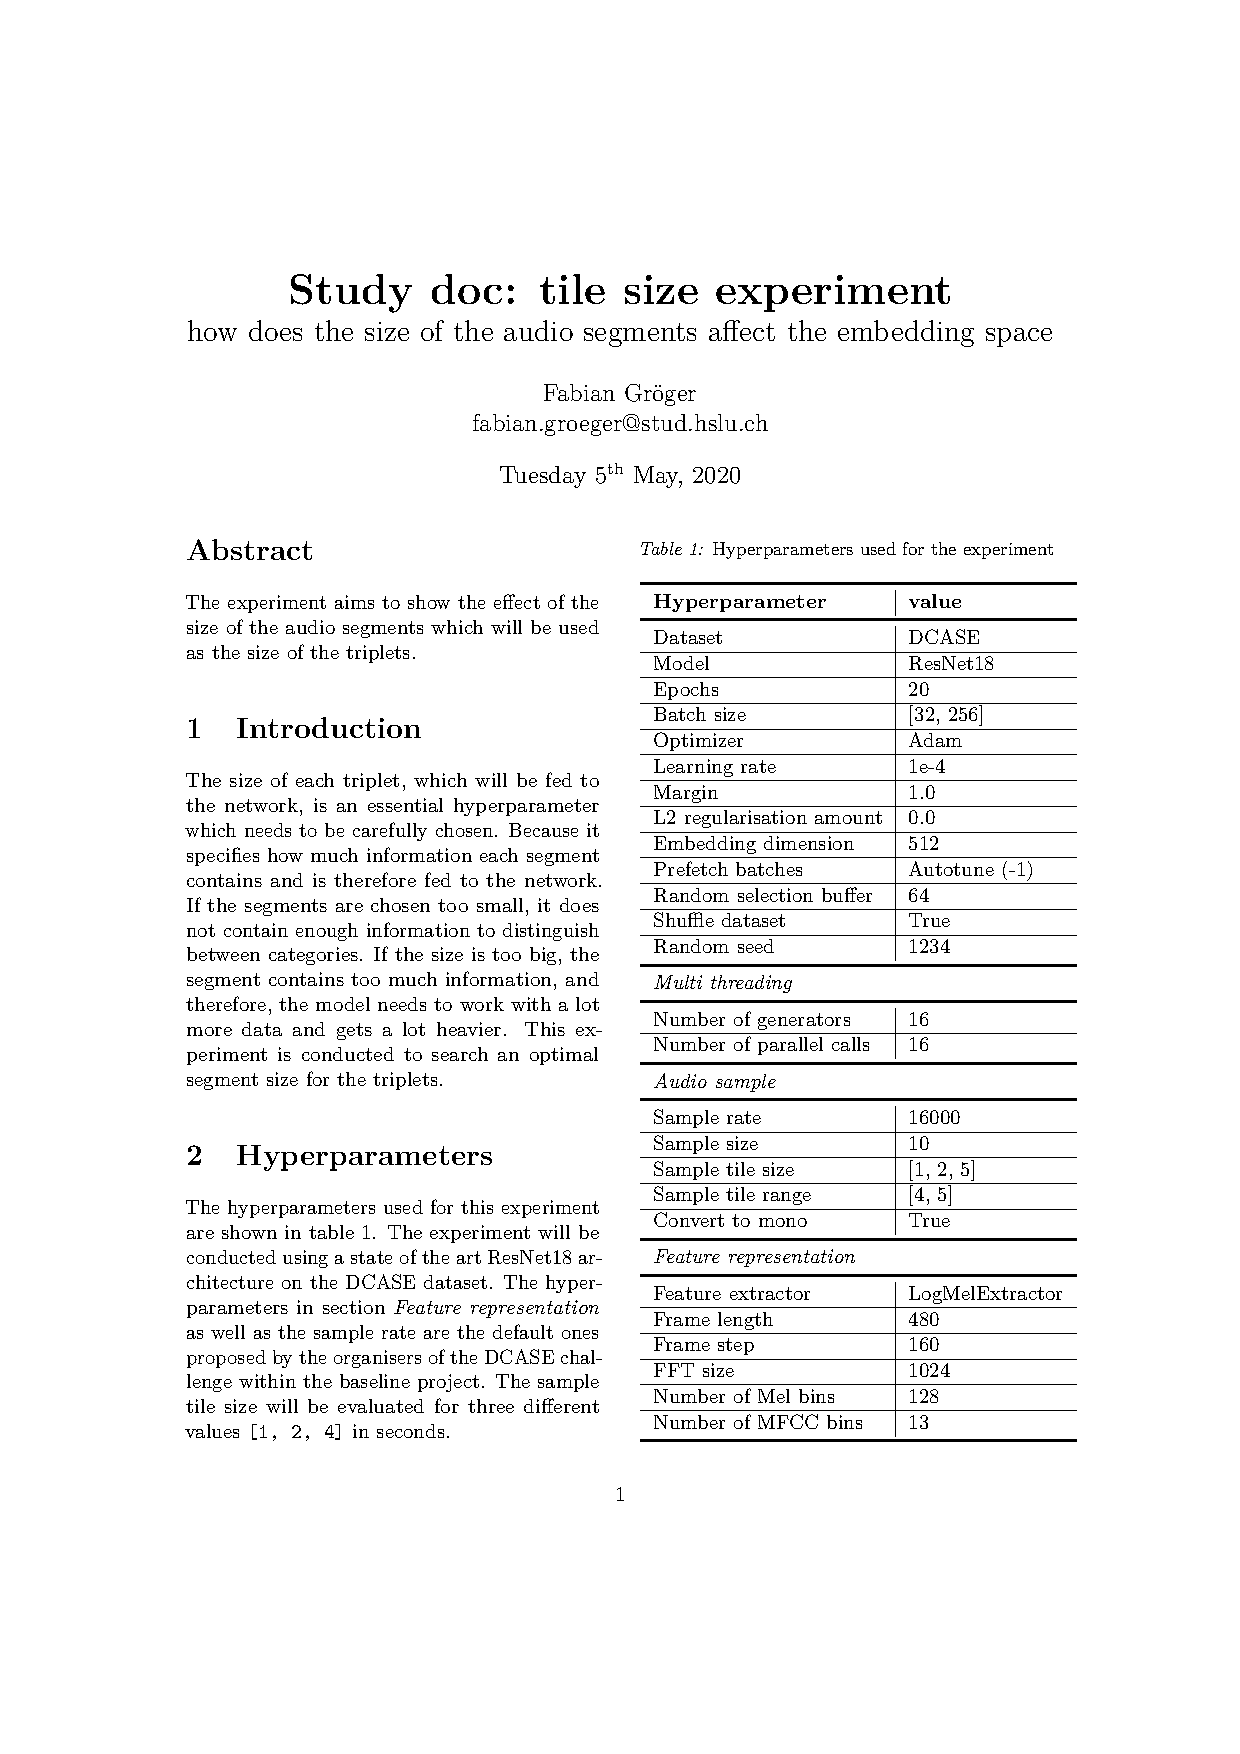
\includepdf[scale=1.0, pages=1-]{study-doc/experiment_tile_size/Study_Doc_tile_size.pdf}

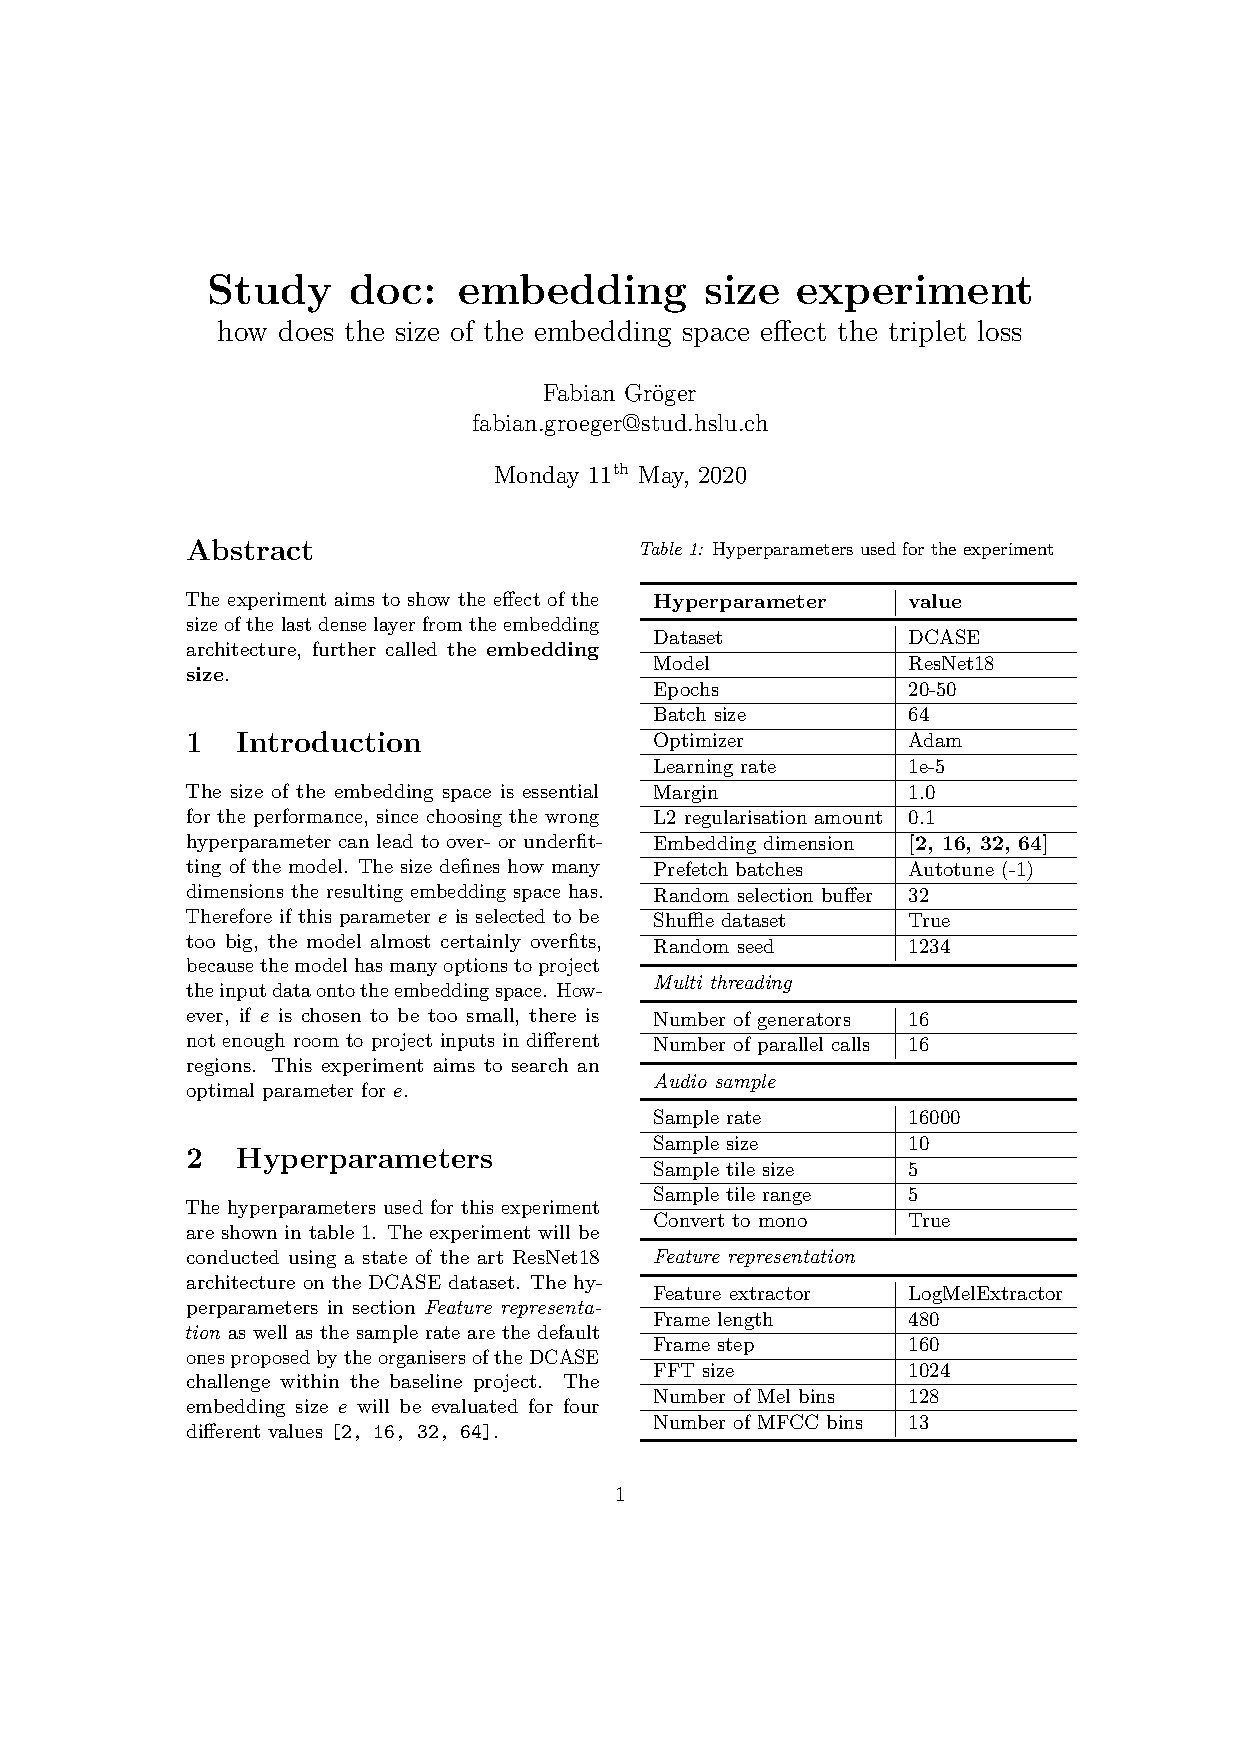
\includepdf[scale=1.0, pages=1-]{study-doc/experiment_embedding_size/Study_Doc_embedding_size.pdf}

\chapter{Work journal}
\label{app:Work-Journal}

Within this chapter, the whole work journal of the thesis is shown. The journal is divided into subcategories, so that the \fullref{tab:Work-Journal} is more pleased to read. These categories show what exactly was done in the different project phases, which can be seen in the \fullref{fig:Project-Plan}. There is also one more category called \flqq General\frqq, where all the administrative tasks are shown, including the meetings with the advisor.

\clearpage
\landscapevalues

\begin{longtable}{| p{.10\textwidth} | p{.20\textwidth} | p{.50\textwidth} | p{.10\textwidth} |} 
	\caption{Work Journal}
	\label{tab:Work-Journal} \\
    \hline
    \textbf{Date} &
    \textbf{Task} &
    \textbf{Details} &
    \textbf{No. hours} \\
    \hline
    \multicolumn{4}{|l|}{\textbf{General}} \\
    \hline
    17.02.2020 & Preparation for Kick-Off Meeting & 
        \begin{minipage}{5in}
        \vskip 4pt
        \begin{itemize}
        \setlength\itemsep{0em}
        \item thesis description read carefully again
        \item questions of unclear matters
        \end{itemize}
        \vskip 4pt
        \end{minipage}
        & 1h  \\
    \hline
    17.02.2020 & Kick-Off Meeting (number 1)& 
        \begin{minipage}{5in}
        \vskip 4pt
        \begin{itemize}
        \setlength\itemsep{0em}
        \item discussed different topics which are important for the implementation of the project
        \end{itemize}
        \vskip 4pt
        \end{minipage}
        & 1h 30min  \\
    \hline
    24.02.2020 & Meeting (number 2) & 
        \begin{minipage}{5in}
        \vskip 4pt
        \begin{itemize}
        \setlength\itemsep{0em}
        \item preparation of the meeting
        \item meeting itself
        \end{itemize}
        \vskip 4pt
        \end{minipage}
        & 2h  \\
    \hline
    02.03.2020 & Meeting (number 3) & 
        \begin{minipage}{5in}
        \vskip 4pt
        \begin{itemize}
        \setlength\itemsep{0em}
        \item preparation of the meeting
        \item meeting itself
        \end{itemize}
        \vskip 4pt
        \end{minipage}
        & 2h  \\
    \hline
    02.03.2020 & Meeting GPU with Thomas Koller & 
        \begin{minipage}{5in}
        \vskip 4pt
        \begin{itemize}
        \setlength\itemsep{0em}
        \item preparation of the meeting
        \item meeting itself
        \end{itemize}
        \vskip 4pt
        \end{minipage}
        & 0.5h  \\
    \hline
    09.03.2020 & Meeting (number 4) & 
        \begin{minipage}{5in}
        \vskip 4pt
        \begin{itemize}
        \setlength\itemsep{0em}
        \item preparation of the meeting
        \item meeting itself
        \end{itemize}
        \vskip 4pt
        \end{minipage}
        & 2h  \\
    \hline
    16.03.2020 & Meeting (number 5) & 
        \begin{minipage}{5in}
        \vskip 4pt
        \begin{itemize}
        \setlength\itemsep{0em}
        \item preparation of the meeting
        \item meeting itself
        \end{itemize}
        \vskip 4pt
        \end{minipage}
        & 2h  \\
    \hline
    23.03.2020 & Meeting (number 6) & 
        \begin{minipage}{5in}
        \vskip 4pt
        \begin{itemize}
        \setlength\itemsep{0em}
        \item preparation of the meeting
        \item meeting itself
        \end{itemize}
        \vskip 4pt
        \end{minipage}
        & 2h  \\
    \hline
    30.03.2020 & Meeting (number 7) & 
        \begin{minipage}{5in}
        \vskip 4pt
        \begin{itemize}
        \setlength\itemsep{0em}
        \item preparation of the meeting
        \item meeting itself
        \end{itemize}
        \vskip 4pt
        \end{minipage}
        & 2h  \\
    \hline
    06.04.2020 & Meeting (number 8) & 
        \begin{minipage}{5in}
        \vskip 4pt
        \begin{itemize}
        \setlength\itemsep{0em}
        \item preparation of the meeting
        \item meeting itself
        \end{itemize}
        \vskip 4pt
        \end{minipage}
        & 2h  \\
    \hline
    15.04.2020 & Meeting (number 9) & 
        \begin{minipage}{5in}
        \vskip 4pt
        \begin{itemize}
        \setlength\itemsep{0em}
        \item preparation of the meeting
        \item meeting itself
        \end{itemize}
        \vskip 4pt
        \end{minipage}
        & 2h  \\
    \hline
    \multicolumn{4}{|l|}{\textbf{Documentation}} \\
    \hline
    17.02.2020 & Documentation setup & 
        \begin{minipage}{5in}
        \vskip 4pt
        \begin{itemize}
        \setlength\itemsep{0em}
        \item project setup
        \item latex document setup
        \item German transcribed to English
        \item built default documentation structure
        \end{itemize}
        \vskip 4pt
        \end{minipage}
        & 2h  \\
    \hline
    19.02.2020 & Dataset documented & 
        \begin{minipage}{5in}
        \vskip 4pt
        \begin{itemize}
        \setlength\itemsep{0em}
        \item SINS Database
        \item DCASE Task dataset
        \end{itemize}
        \vskip 4pt
        \end{minipage}
        & 3h  \\
    \hline
    24.02.2020 & Dataset section finished & 
        \begin{minipage}{5in}
        \vskip 4pt
        \begin{itemize}
        \setlength\itemsep{0em}
        \item Created table of the recorded activities in the \gls{SINS} database
        \item Reread section and corrected
        \end{itemize}
        \vskip 4pt
        \end{minipage}
        & 1h  \\
    \hline
    02.03.2020 & Triplet Loss section finished & 
        \begin{minipage}{5in}
        \vskip 4pt
        \begin{itemize}
        \setlength\itemsep{0em}
        \item Documented Triplet Loss in related work
        \item Reread section and corrected
        \end{itemize}
        \vskip 4pt
        \end{minipage}
        & 2h  \\
    \hline
    03.03.2020 & Tile2Vec section finished & 
        \begin{minipage}{5in}
        \vskip 4pt
        \begin{itemize}
        \setlength\itemsep{0em}
        \item Documented Tile2Vec in related work
        \item Reread section and corrected
        \item Corrected equations
        \end{itemize}
        \vskip 4pt
        \end{minipage}
        & 2h  \\
    \hline
    05.03.2020 & Started with intro to neural networks & 
        \begin{minipage}{5in}
        \vskip 4pt
        \begin{itemize}
        \setlength\itemsep{0em}
        \item Researched neural networks
        \item Documented neural networks
        \end{itemize}
        \vskip 4pt
        \end{minipage}
        & 4h  \\
    \hline
    06.03.2020 & Finished with intro to neural networks & 
        \begin{minipage}{5in}
        \vskip 4pt
        \begin{itemize}
        \setlength\itemsep{0em}
        \item Documented neural networks
        \end{itemize}
        \vskip 4pt
        \end{minipage}
        & 4h  \\
    \hline
    05.03.2020 & Started with intro to convolutional neural networks & 
        \begin{minipage}{5in}
        \vskip 4pt
        \begin{itemize}
        \setlength\itemsep{0em}
        \item Researched convolutional neural networks
        \item Documented convolutional neural networks
        \end{itemize}
        \vskip 4pt
        \end{minipage}
        & 2h  \\
    \hline
    09.03.2020 & Finished intro to convolutional neural networks & 
        \begin{minipage}{5in}
        \vskip 4pt
        \begin{itemize}
        \setlength\itemsep{0em}
        \item Documented convolutional neural networks
        \end{itemize}
        \vskip 4pt
        \end{minipage}
        & 3h  \\
    \hline
    09.03.2020 & Documented various parts & 
        \begin{minipage}{5in}
        \vskip 4pt
        \begin{itemize}
        \setlength\itemsep{0em}
        \item Documented project plan and milestones
        \item Documented introduction
        \item Documented appendix
        \item Documented into to clustering
        \end{itemize}
        \vskip 4pt
        \end{minipage}
        & 3h  \\
    \hline
    11.03.2020 & Document changes applied from meeting & 
        \begin{minipage}{5in}
        \vskip 4pt
        \begin{itemize}
        \setlength\itemsep{0em}
        \item Moving Dataset to related work
        \item Changed denotation of loss function
        \item Changed NN section
        \end{itemize}
        \vskip 4pt
        \end{minipage}
        & 1h  \\
    \hline
    11.03.2020 & Finished intro to gated recurrent unit & 
        \begin{minipage}{5in}
        \vskip 4pt
        \begin{itemize}
        \setlength\itemsep{0em}
        \item Documented gated recurrent unit
        \end{itemize}
        \vskip 4pt
        \end{minipage}
        & 2h  \\
    \hline
    13.03.2020 & Finished status in relation to project & 
        \begin{minipage}{5in}
        \vskip 4pt
        \begin{itemize}
        \setlength\itemsep{0em}
        \item Researched state-of-the-art in audio deep learning
        \item Documented status in relation to project
        \end{itemize}
        \vskip 4pt
        \end{minipage}
        & 4h  \\
    \hline
    15.03.2020 & Finished related work & 
        \begin{minipage}{5in}
        \vskip 4pt
        \begin{itemize}
        \setlength\itemsep{0em}
        \item Researched dilated convolution
        \item Documented dilated convolution
        \end{itemize}
        \vskip 4pt
        \end{minipage}
        & 2h  \\
    \hline
    15.03.2020 & Milestone review & 
        \begin{minipage}{5in}
        \vskip 4pt
        \begin{itemize}
        \setlength\itemsep{0em}
        \item M1 milestone review
        \end{itemize}
        \vskip 4pt
        \end{minipage}
        & 1h  \\
    \hline
    27.03.2020 & Started with changes from Daniel & 
        \begin{minipage}{5in}
        \vskip 4pt
        \begin{itemize}
        \setlength\itemsep{0em}
        \item Related Work changes
        \end{itemize}
        \vskip 4pt
        \end{minipage}
        & 2h  \\
    \hline
    28.03.2020 & Started with chapter 3, Ideas and concepts & 
        \begin{minipage}{5in}
        \vskip 4pt
        \begin{itemize}
        \setlength\itemsep{0em}
        \item Data preprocessing
        \item Feature extraction
        \item Data augmentation
        \end{itemize}
        \vskip 4pt
        \end{minipage}
        & 3h  \\
    \hline
    29.03.2020 & Milestone review & 
        \begin{minipage}{5in}
        \vskip 4pt
        \begin{itemize}
        \setlength\itemsep{0em}
        \item M2 milestone review
        \end{itemize}
        \vskip 4pt
        \end{minipage}
        & 1h  \\
    \hline
    06.04.2020 & Finished with changes from Daniel & 
        \begin{minipage}{5in}
        \vskip 4pt
        \begin{itemize}
        \setlength\itemsep{0em}
        \item Related Work changes
        \end{itemize}
        \vskip 4pt
        \end{minipage}
        & 1h  \\
    \hline
    06.04.2020 & Worked on chapter 3, Ideas and concepts & 
        \begin{minipage}{5in}
        \vskip 4pt
        \begin{itemize}
        \setlength\itemsep{0em}
        \item Input pipeline
        \item Triplet selection
        \item refactoring of chapter
        \end{itemize}
        \vskip 4pt
        \end{minipage}
        & 3h 30min  \\
    \hline
    12.04.2020 & Milestone review & 
        \begin{minipage}{5in}
        \vskip 4pt
        \begin{itemize}
        \setlength\itemsep{0em}
        \item M3 milestone review
        \end{itemize}
        \vskip 4pt
        \end{minipage}
        & 1h  \\
    \hline
    13.04.2020 & Worked on chapter 3, Ideas and concepts & 
        \begin{minipage}{5in}
        \vskip 4pt
        \begin{itemize}
        \setlength\itemsep{0em}
        \item Rewrote most of the sections
        \item Finished draft of chapter 3
        \end{itemize}
        \vskip 4pt
        \end{minipage}
        & 3h \\
    \hline
    13.04.2020 & Worked on chapter 4, Method &
        \begin{minipage}{5in}
        \vskip 4pt
        \begin{itemize}
        \setlength\itemsep{0em}
        \item Updated project plan
        \item Started with documentation of procedure model
        \end{itemize}
        \vskip 4pt
        \end{minipage}
        & 1h \\
    \hline
    15.04.2020 & Worked on interim presentation &
        \begin{minipage}{5in}
        \vskip 4pt
        \begin{itemize}
        \setlength\itemsep{0em}
        \item Created slides
        \item Reviewed slides
        \end{itemize}
        \vskip 4pt
        \end{minipage}
        & 4h \\
    \hline
    16.04.2020 & Worked on interim presentation &
        \begin{minipage}{5in}
        \vskip 4pt
        \begin{itemize}
        \setlength\itemsep{0em}
        \item Practised presentation
        \end{itemize}
        \vskip 4pt
        \end{minipage}
        & 4h \\
    \hline
    20.04.2020 & Worked on interim presentation &
        \begin{minipage}{5in}
        \vskip 4pt
        \begin{itemize}
        \setlength\itemsep{0em}
        \item Practised presentation
        \end{itemize}
        \vskip 4pt
        \end{minipage}
        & 2h \\
    \hline
    24.04.2020 & Worked on chapter 4, Method &
        \begin{minipage}{5in}
        \vskip 4pt
        \begin{itemize}
        \setlength\itemsep{0em}
        \item Project structure
        \item Resources
        \item Evaluation
        \end{itemize}
        \vskip 4pt
        \end{minipage}
        & 6h \\
    \hline
    \multicolumn{4}{|l|}{\textbf{Research}} \\
    \hline
    17.02.2020 & Research Dataset & 
        \begin{minipage}{5in}
        \vskip 4pt
        \begin{itemize}
        \setlength\itemsep{0em}
        \item finished with DCASE - Challenge description
        \item started with SINS Database Paper
        \end{itemize}
        \vskip 4pt
        \end{minipage}
        & 2h 30min  \\
    \hline
    21.02.2020 & Audio processing research & 
        \begin{minipage}{5in}
        \vskip 4pt
        \begin{itemize}
        \setlength\itemsep{0em}
        \item \gls{FT}
        \item \gls{FFT}
        \item \gls{DFT}
        \item Spectrogram
        \item started with related work documentation
        \end{itemize}
        \vskip 4pt
        \end{minipage}
        & 5h  \\
    \hline
    26.02.2020 & Audio processing research & 
        \begin{minipage}{5in}
        \vskip 4pt
        \begin{itemize}
        \setlength\itemsep{0em}
        \item \gls{MFCC}
        \item documenting research in related work
        \end{itemize}
        \vskip 4pt
        \end{minipage}
        & 3h  \\
    \hline
    27.02.2020 & Audio processing research & 
        \begin{minipage}{5in}
        \vskip 4pt
        \begin{itemize}
        \setlength\itemsep{0em}
        \item \gls{MFCC}
        \item finished documenting research in related work
        \end{itemize}
        \vskip 4pt
        \end{minipage}
        & 4h  \\
    \hline
    28.02.2020 & Triplet Loss research & 
        \begin{minipage}{5in}
        \vskip 4pt
        \begin{itemize}
        \setlength\itemsep{0em}
        \item read various paper on triplet loss
        \end{itemize}
        \vskip 4pt
        \end{minipage}
        & 3h  \\
    \hline
    01.03.2020 & Triplet Loss research & 
        \begin{minipage}{5in}
        \vskip 4pt
        \begin{itemize}
        \setlength\itemsep{0em}
        \item current research on triplet loss with audio
        \end{itemize}
        \vskip 4pt
        \end{minipage}
        & 2h  \\
    \hline
    02.03.2020 & Tile2Vec research & 
        \begin{minipage}{5in}
        \vskip 4pt
        \begin{itemize}
        \setlength\itemsep{0em}
        \item read various paper on tile2vec
        \item started documenting tile2vec in related work
        \end{itemize}
        \vskip 4pt
        \end{minipage}
        & 5h  \\
    \hline
    \multicolumn{4}{|l|}{\textbf{Realisation}} \\
    \hline
    14.03.2020 & Started with project setup and input pipeline & 
        \begin{minipage}{5in}
        \vskip 4pt
        \begin{itemize}
        \setlength\itemsep{0em}
        \item set up the GitHub project
        \item started with input pipeline
        \item generator of triplets
        \end{itemize}
        \vskip 4pt
        \end{minipage}
        & 8h  \\
    \hline
    15.03.2020 & Started with input pipeline & 
        \begin{minipage}{5in}
        \vskip 4pt
        \begin{itemize}
        \setlength\itemsep{0em}
        \item first test cases for input pipeline
        \item implemented first idea of similarity measure between audios
        \end{itemize}
        \vskip 4pt
        \end{minipage}
        & 2h  \\
    \hline
    16.03.2020 & Input pipeline finished & 
        \begin{minipage}{5in}
        \vskip 4pt
        \begin{itemize}
        \setlength\itemsep{0em}
        \item finished input pipeline
        \item finished unit test for pipeline
        \end{itemize}
        \vskip 4pt
        \end{minipage}
        & 7h  \\
    \hline
    18.03.2020 & Project setup & 
        \begin{minipage}{5in}
        \vskip 4pt
        \begin{itemize}
        \setlength\itemsep{0em}
        \item finished project structure
        \end{itemize}
        \vskip 4pt
        \end{minipage}
        & 2h  \\
    \hline
    18.03.2020 & Implementation & 
        \begin{minipage}{5in}
        \vskip 4pt
        \begin{itemize}
        \setlength\itemsep{0em}
        \item Triplet loss implemented
        \item Dense model implemented
        \item Started with projector visualisation
        \end{itemize}
        \vskip 4pt
        \end{minipage}
        & 5h  \\
    \hline
    20.03.2020 & Implementation & 
        \begin{minipage}{5in}
        \vskip 4pt
        \begin{itemize}
        \setlength\itemsep{0em}
        \item Train workflow implemented
        \end{itemize}
        \vskip 4pt
        \end{minipage}
        & 5h  \\
    \hline
    23.03.2020 & Implementation & 
        \begin{minipage}{5in}
        \vskip 4pt
        \begin{itemize}
        \setlength\itemsep{0em}
        \item Tested models and workflow on GPU
        \item Convolutional model implemented
        \end{itemize}
        \vskip 4pt
        \end{minipage}
        & 5h  \\
    \hline
    25.03.2020 & Implementation & 
        \begin{minipage}{5in}
        \vskip 4pt
        \begin{itemize}
        \setlength\itemsep{0em}
        \item Convolutional model edited (1D and 2D)
        \item Training workflow edited
        \end{itemize}
        \vskip 4pt
        \end{minipage}
        & 4h  \\
    \hline
    27.03.2020 & Implementation & 
        \begin{minipage}{5in}
        \vskip 4pt
        \begin{itemize}
        \setlength\itemsep{0em}
        \item Factories implemented
        \item Metrics implemented
        \end{itemize}
        \vskip 4pt
        \end{minipage}
        & 5h  \\
    \hline
    31.03.2020 & Implementation & 
        \begin{minipage}{5in}
        \vskip 4pt
        \begin{itemize}
        \setlength\itemsep{0em}
        \item GRU Model implemented
        \item refactoring
        \end{itemize}
        \vskip 4pt
        \end{minipage}
        & 4h  \\
    \hline
    03.04.2020 & Implementation & 
        \begin{minipage}{5in}
        \vskip 4pt
        \begin{itemize}
        \setlength\itemsep{0em}
        \item Music dataset pipeline
        \item Unit tests finished
        \item Documentation of code
        \item Worked on Classifier
        \end{itemize}
        \vskip 4pt
        \end{minipage}
        & 6h  \\
    \hline
    04.04.2020 & Implementation & 
        \begin{minipage}{5in}
        \vskip 4pt
        \begin{itemize}
        \setlength\itemsep{0em}
        \item Worked on evaluation workflow
        \end{itemize}
        \vskip 4pt
        \end{minipage}
        & 3h  \\
    \hline
    07.04.2020 & Implementation & 
        \begin{minipage}{5in}
        \vskip 4pt
        \begin{itemize}
        \setlength\itemsep{0em}
        \item Input pipeline multiprocessing
        \end{itemize}
        \vskip 4pt
        \end{minipage}
        & 5h  \\
    \hline
    08.04.2020 & Implementation & 
        \begin{minipage}{5in}
        \vskip 4pt
        \begin{itemize}
        \setlength\itemsep{0em}
        \item Changed triplet selection of datasets
        \end{itemize}
        \vskip 4pt
        \end{minipage}
        & 6h  \\
    \hline
    12.04.2020 & Implementation & 
        \begin{minipage}{5in}
        \vskip 4pt
        \begin{itemize}
        \setlength\itemsep{0em}
        \item Finished evaluation workflow
        \item Added new metrics to classifier
        \end{itemize}
        \vskip 4pt
        \end{minipage}
        & 4h  \\
    \hline
    14.04.2020 & Implementation & 
        \begin{minipage}{5in}
        \vskip 4pt
        \begin{itemize}
        \setlength\itemsep{0em}
        \item Input pipeline speedup
        \end{itemize}
        \vskip 4pt
        \end{minipage}
        & 3h  \\
    \hline
    15.04.2020 & Implementation & 
        \begin{minipage}{5in}
        \vskip 4pt
        \begin{itemize}
        \setlength\itemsep{0em}
        \item Added ResNet architecture
        \end{itemize}
        \vskip 4pt
        \end{minipage}
        & 4h  \\
    \hline
    \multicolumn{4}{|l|}{\textbf{Experiments}} \\
    \hline
    17.03.2020 & Started with first experiment & 
        \begin{minipage}{5in}
        \vskip 4pt
        \begin{itemize}
        \setlength\itemsep{0em}
        \item margin experiment
        \end{itemize}
        \vskip 4pt
        \end{minipage}
        & 5h  \\
    \hline
    22.03.2020 & Finished with first experiment & 
        \begin{minipage}{5in}
        \vskip 4pt
        \begin{itemize}
        \setlength\itemsep{0em}
        \item margin experiment
        \end{itemize}
        \vskip 4pt
        \end{minipage}
        & 5h  \\
    \hline
    23.03.2020 & Started with experiment & 
        \begin{minipage}{5in}
        \vskip 4pt
        \begin{itemize}
        \setlength\itemsep{0em}
        \item feature representation
        \end{itemize}
        \vskip 4pt
        \end{minipage}
        & 3h  \\
    \hline
\end{longtable}

\clearpage
\defaultpagestyle

\chapter{Task definition bachelor thesis}
\label{app:Task-Definition}

Within this chapter the final task definition, which was submitted and accepted by the Transfer Office of the Lucerne University of Applied Sciences and Arts on the 25.02.2020, is attached.

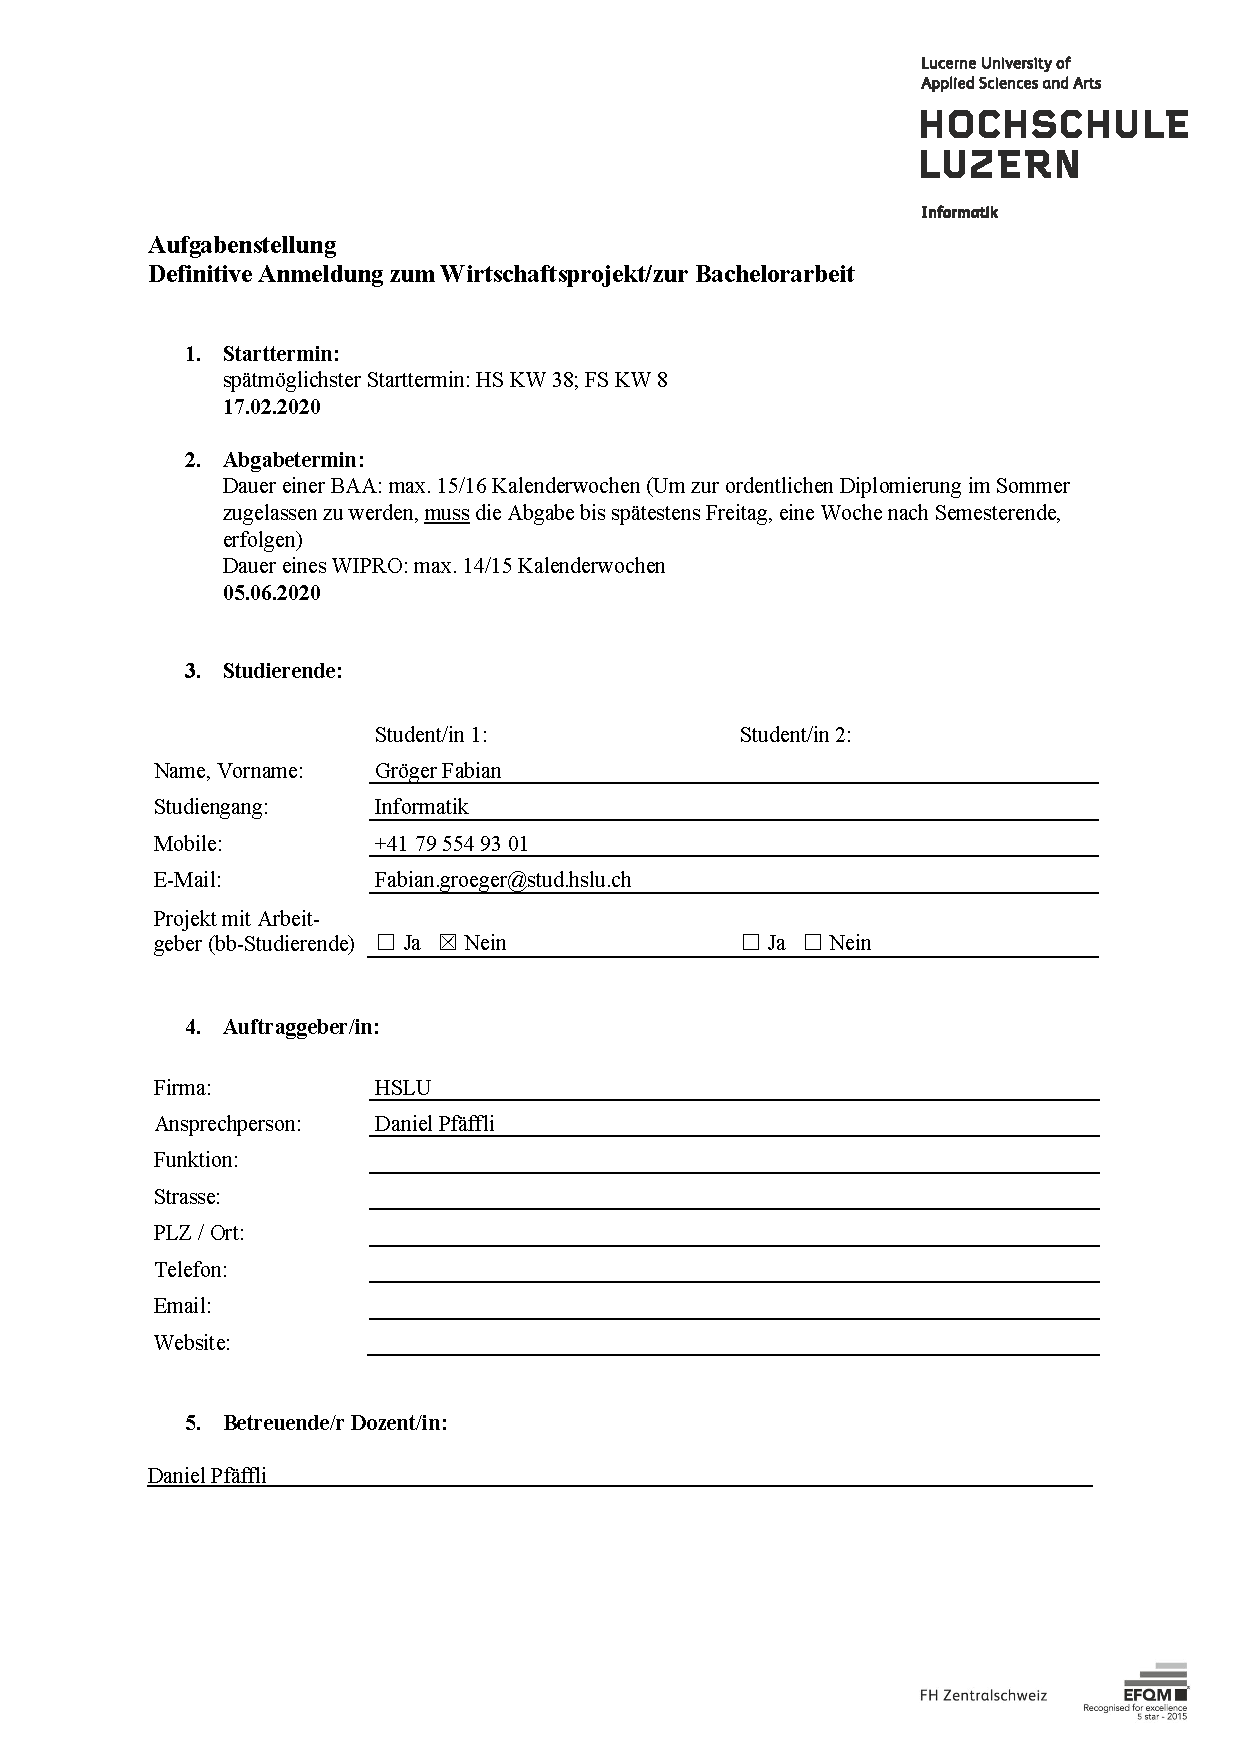
\includepdf[scale=1.0, pages=1-]{files/Aufgabenstellung_DeepEmbeddedMusic.pdf}
